\documentclass[tikz]{standalone}

\usepackage{tikz}
\usepackage{tcolorbox}
\usepackage{pagecolor}
\usepackage{amsmath}
\usepackage{color}
\usepackage{blkarray}
\usepackage{graphicx}

\definecolor{mygray}{gray}{0.7}
\pagecolor{white}


\begin{document}
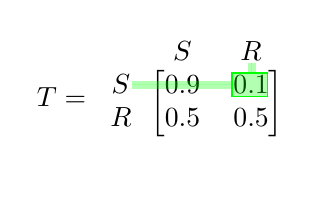
\begin{tikzpicture}

\node (A) at (-0.5,  0.2) {};
\node (B) at (1.02,  0.2) {};
\node (C) at (1.15 ,   .235) {};
\node (D) at (1.15 , .6) {};
\node (E) at (.9 ,  0.35) {};
\node (F) at (1.35 , .05) {};


\node (0) [] at (0, 0) {$T=
\begin{blockarray}{ccc}
& S & R \\
\begin{block}{c[cc]}
    S & 0.9 & 0.1 \\
    R & 0.5 & 0.5 \\
\end{block}
\end{blockarray}
$};

\draw [line width=1mm,
    draw=green,
    fill=green,
    draw opacity=.3]
    (A) -- (B) (C) -- (D);

\draw[fill=green, fill opacity = .3, draw=green] (E) rectangle (F);


\end{tikzpicture}
\end{document}
